%%---------------------------------------------------------------------------%%
%% NSE Article
%% 2013: RQI+MGE
%%---------------------------------------------------------------------------%%

\documentclass[12pt]{article}
\usepackage{amsmath}
\usepackage{amssymb,amsthm,graphicx}
\usepackage{epsfig}
\usepackage[mathcal]{euscript}
%\usepackage{citesort}
\usepackage{setspace}
%\usepackage{tmadd,tmath}
\usepackage{color}
\usepackage{array}
%\usepackage{c++}
%\usepackage{times, mathptm}
\usepackage{subfigure}
%\usepackage{dsfont}

\usepackage{times}
\renewcommand{\ttdefault}{cmtt}

\usepackage{fancyhdr} % used to put page number in header instead of footer

% The float package HAS to load before hyperref
\usepackage{float} % for psuedocode formatting
\usepackage{xspace}

% from Denovo Methods Manual
\usepackage{mathrsfs}

\usepackage[pdftex]{hyperref}
% define a style for pseudocode. This must load AFTER hyperref.
\floatstyle{ruled}
\newfloat{algorithm}{h}{lop}
\floatname{algorithm}{Algorithm}


%%---------------------------------------------------------------------------%%

%\setlength{\textfloatsep}{8pt plus 1pt minus 1pt}
%\setlength{\abovedisplayskip}{4pt plus 1pt minus 1pt}
%\setlength{\belowdisplayskip}{4pt plus 1pt minus 1pt}
%\addtolength{\oddsidemargin}{-0.5in}
%\addtolength{\textwidth}{1.0in}
%\addtolength{\textheight}{0.5in}

\setlength{\textwidth}{6.5in}
\setlength{\oddsidemargin}{0.0in}
\setlength{\evensidemargin}{0.0in}
\setlength{\textheight}{9.0in}
\setlength{\topmargin}{0.0in}
\setlength{\headheight}{0.0in}
\setlength{\headsep}{0.0in}
\setlength{\footskip}{0.5in}

\renewcommand{\thefootnote}{\fnsymbol{footnote}}
\renewcommand{\thetable}{\Roman{table}}

%%---------------------------------------------------------------------------%%

\newcommand{\email}[1]{$\langle$#1@pitt.edu$\rangle$}

\DeclareMathOperator{\diag}{diag}
\DeclareMathOperator{\low}{lower}
\DeclareMathOperator{\upp}{upper}

\newcommand{\SN}{\ensuremath{S_N}}
\newcommand{\Macro}{\ensuremath{\Sigma}}

\newcommand{\vOmega}{\ensuremath{\hat{\Omega}}}
\newcommand{\Ye}[2]{\ensuremath{Y^e_{#1}(\vOmega_#2)}}
\newcommand{\Yo}[2]{\ensuremath{Y^o_{#1}(\vOmega_#2)}}

\newcommand{\ve}[1]{\ensuremath{\mathbf{#1}}}

\newcommand{\sigg}[1]{\ensuremath{\sigma^{gg'}_{\text{s}\,#1}}}
\newcommand{\psig}{\ensuremath{\psi^g}}

\newcommand{\even}{\ensuremath{\phi^g}}
\newcommand{\odd}{\ensuremath{\vartheta^g}}

\newcommand{\evenp}{\ensuremath{\phi^{g'}}}
\newcommand{\oddp}{\ensuremath{\vartheta^{g'}}}

\newcommand{\apsi}[1]{\ensuremath{\psi^{\dagger\,#1}}}
\newcommand{\aeven}[1]{\ensuremath{\phi^{\dagger\,#1}}}
\newcommand{\aodd}[1]{\ensuremath{\vartheta^{\dagger\,#1}}}
\newcommand{\asigg}[1]{\ensuremath{\sigma^{g'g}_{\text{s}\,#1}}}

\newcommand{\aPsi}[1]{\ensuremath{\Psi^{\dagger\,#1}}}
\newcommand{\aPhi}[1]{\ensuremath{\Phi^{\dagger\,#1}}}

\newcommand{\epsi}{\ensuremath{\epsilon}}
\newcommand{\ephi}{\ensuremath{\varepsilon}}

\newcommand{\psie}{\ensuremath{\psi_{\epsi}}}
\newcommand{\phie}{\ensuremath{\phi_{\ephi}}}

\newcommand{\Psie}{\ensuremath{\Psi_{\epsi}}}
\newcommand{\Phie}{\ensuremath{\Phi_{\ephi}}}

\newcommand{\apsie}[1]{\ensuremath{\psi^{\dagger\,#1}_{\epsi}}}
\newcommand{\aphie}[1]{\ensuremath{\phi^{\dagger\,#1}_{\ephi}}}

\newcommand{\aPsie}[1]{\ensuremath{\Psi^{\dagger\,#1}_{\epsi}}}
\newcommand{\aPhie}[1]{\ensuremath{\Phi^{\dagger\,#1}_{\ephi}}}

\newcommand{\avg}[1]{\ensuremath{\langle#1\rangle}}

\newcommand{\osig}{\ensuremath{\overline{\sigma}}}
\newcommand{\osigs}{\ensuremath{\overline{\sigma_{\text{s}}}}}

%%---------------------------------------------------------------------------%%

\begin{document}

\setcounter{page}{2}
  
%%---------------------------------------------------------------------------%%

\begin{center}

  {\large \bf Title}
  
  \vspace{0.3in}
  
  R.N. Slaybaugh, T.M. Evans, G.G. Davidson, and P.P.H. Wilson
  
\end{center}

\doublespacing

\vspace{0.3in}

\begin{abstract}

  Abstract

\end{abstract}

\newpage

%%---------------------------------------------------------------------------%%

\section{Introduction}

Introduction

%%---------------------------------------------------------------------------%%

\section{Conclusions}
\label{sec:conclusions}

Conclusions

%%---------------------------------------------------------------------------%%

\section{Acknowledgements}

This research used resources of the Oak Ridge Leadership Computing Facility at the Oak Ridge National Laboratory, which is supported by the Office of Science of the U.S. Department of Energy under Contract No. DE-AC05-00OR22725. Additional thanks to the Rickover Fellowship Program in Nuclear Engineering sponsored by Naval Reactors Division of the U.S. Department of Energy. This fellowship sponsored the work from which this work is derived. 

%%---------------------------------------------------------------------------%%

\newpage
\appendix

\section{Angular Flux Moments}
\label{sec:angular-flux-moments}

Appendix

%%---------------------------------------------------------------------------%%
%% BIBLIOGRAPHY
%%---------------------------------------------------------------------------%%

\newpage

\singlespacing

\bibliographystyle{jcp}
\bibliography{RQI_MGE}

%%---------------------------------------------------------------------------%%
%% TABLES
%%---------------------------------------------------------------------------%%

\clearpage

\begin{table}[p]
  \caption{
    Comparison of results for the adjoint neutron porosity tool
    problem. For these problems, the adjoint source is place in the
    far detector.  All timing results are normalized to the
    unaccelerated Gauss-Seidel iteration time.
  }
  \label{tab:adjoint-porosity-tool}
  \begin{center}
    \begin{tabular}{lcll}\hline\hline
      Method & Acceleration $S_N$ order & GS iterations & Time \\\hline
      %%
      GS & - & 53 & 1.0   \\
      TTG & 8 & 7 & 0.172 \\
      TTG & 2 & 7 & 0.159 \\
      \hline\hline
    \end{tabular}
  \end{center}
\end{table}

%%---------------------------------------------------------------------------%%

\clearpage

\begin{table}[p]
  \caption{
    Results from the neutron porosity tool problem using MTTG.  All
    timing results are normalized to the unaccelerated Gauss-Seidel
    iteration time.
  }
  \label{tab:MTTG-porosity-tool}
  \begin{center}
    \begin{tabular}{llllll}\hline\hline
      Method & Acceleration $S_N$  & GS Iterations & Within-group
      & Acceleration & Time \\
      & order & & sweeps & sweeps &  \\\hline
      %%
      GS   & - & 175 & 16294 & 0    & 1.0   \\
      TTG  & 8 & 15  & 1398  & 547  & 0.113 \\
      TTG  & 2 & 13  & 1212  & 459  & 0.086 \\
      MTTG & 2 & 47  & 611   & 1329 & 0.050 \\
      \hline\hline
    \end{tabular}
  \end{center}
\end{table}

%%---------------------------------------------------------------------------%%
%% FIGURES
%%---------------------------------------------------------------------------%%

\clearpage

\begin{figure}[p]
  \begin{center}
    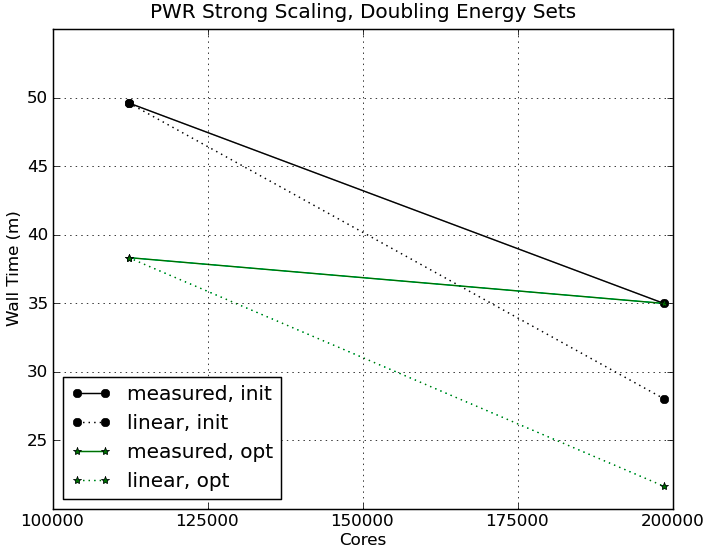
\includegraphics[width=6in,clip]{PWRstrongScaling}
  \end{center}
  \caption{Example1}
  \label{fig:example1}
\end{figure}

%%---------------------------------------------------------------------------%%

\clearpage

\begin{figure}[p]
  \begin{center}
    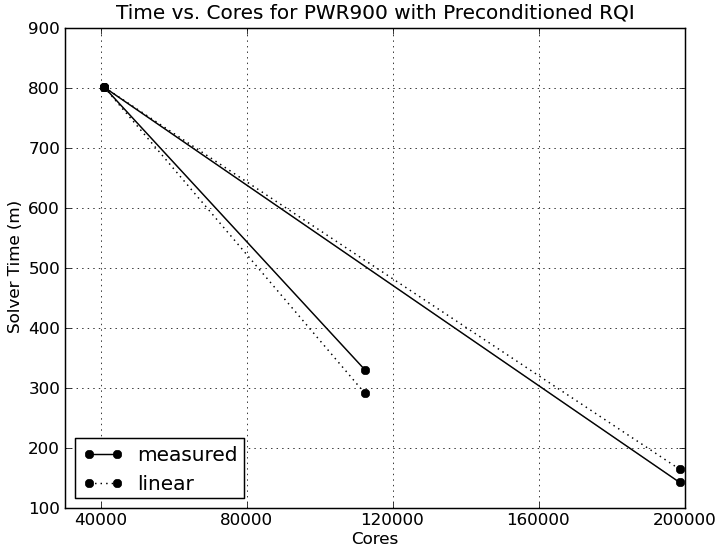
\includegraphics[width=6in,clip]{PWRPrecondRQI}
  \end{center}
  \caption{Example}
  \label{fig:example2}
\end{figure}

%%---------------------------------------------------------------------------%%

\clearpage

\singlespacing
\begin{center}

  {\Large \bf Title}
  
  \vspace{0.3in}
  
  {\large R.N. Slaybaugh\footnote{Corresponding author.  Telephone: +1
      570 850 3385.  E-mail: rns37@pitt.edu.}\\
    Department of Mechanical Engineering and Material Science\\
    University of Pittsburgh\\
    605 Benedum Hall, 3700 O'Hara Street\\
    Pittsburgh, PA 15261, USA\\\vspace{1\baselineskip}
    T.M. Evans, G.G. Davidson\\
    Radiation Transport and Criticality Group\\ 
    Oak Ridge National Laboratory\\ 
    P.O. Box 2008\\
    Oak Ridge, TN 37831-6170, USA\\\vspace{1\baselineskip}
    P.P.H. Wilson\\
    Department of Nuclear Engineering and Engineering Physics\\
    University of Wisconsin - Madison\\
    419 ERB, 1500 Engineering Drive\\
    Madison, WI 52706, USA\\}
  
  \addtocounter{page}{-1}

  \vspace{2.0in}
  \renewcommand{\thetable}{\arabic{table}}
  \thepage\ Pages --- \thetable\ Tables --- \thefigure\ Figures \\

  \setcounter{page}{1}

\end{center}

%%---------------------------------------------------------------------------%%

\end{document}

%%---------------------------------------------------------------------------%%
%% end of paper.tex
%%---------------------------------------------------------------------------%%
